
\section{Louvain Algorithm}
The Louvain algorithm is a greedy modularity optimization technique designed by a team of researcher composed by Vincent D. Blondel, Jean-Loup Guillaume, Renaud Lambiotte and Etienne Lefebvre in the 2008 \cite{Blondel_2008}. The algorithm bears the name of the university to which they belong to, i.e. \textit{Université Catholique de Louvain}.
In 2008, the fastest algorithm presented in the literature was the one proposed by Clauset et al. \cite{Clauset_2004}, but the biggest graph at the time that was analysed has 5.5 million users. This was a not so big graph even at the time. For example, Facebook in 2008 has 64 million active users, more than ten times the size of the biggest analyzed graph. This algorithm was proposed to resolve this scaling problem:  indeed the first version of this algorithm identified communities in a 118 million nodes network in 152 minutes \cite{Blondel_2008}. From that year, many improvements were made and some parallel versions were proposed. 
This algorithm and its parallel version is the main topic of this thesis. The algorithm is very popular due to his simplicity, efficiency and overall precision.
In this chapter, we present the sequential algorithm in details and some optimization technique presented in the literature.
Then we present the parallel version of the algorithm, focusing on the implementations exploiting GPU.
\subsection{Algorithm}
This greedy algorithm is quite simple. There are two phases that are repeated iteratively: the optimization phase and the aggregation phase. At the start of the optimization, given a graph $G(V,E)$, each nodes is assigned to its self-community, i.e. , each node belongs to a community composed by only itself. 
In the first phase, given a node $i\in V$, its community $c_i$ and its neighbourhood $N(i)$, we evaluate, for each community $c_j$ such that $c_j$ has at least one node in $N(i)$, the gain of modularity $\Delta Q_{i \rightarrow c_j}$ that we have if we remove $i$ from its community $c_i$ and we assign it to the community $c_j$. 
\begin{figure}[h]
	\centering
	\hspace*{-1em}
	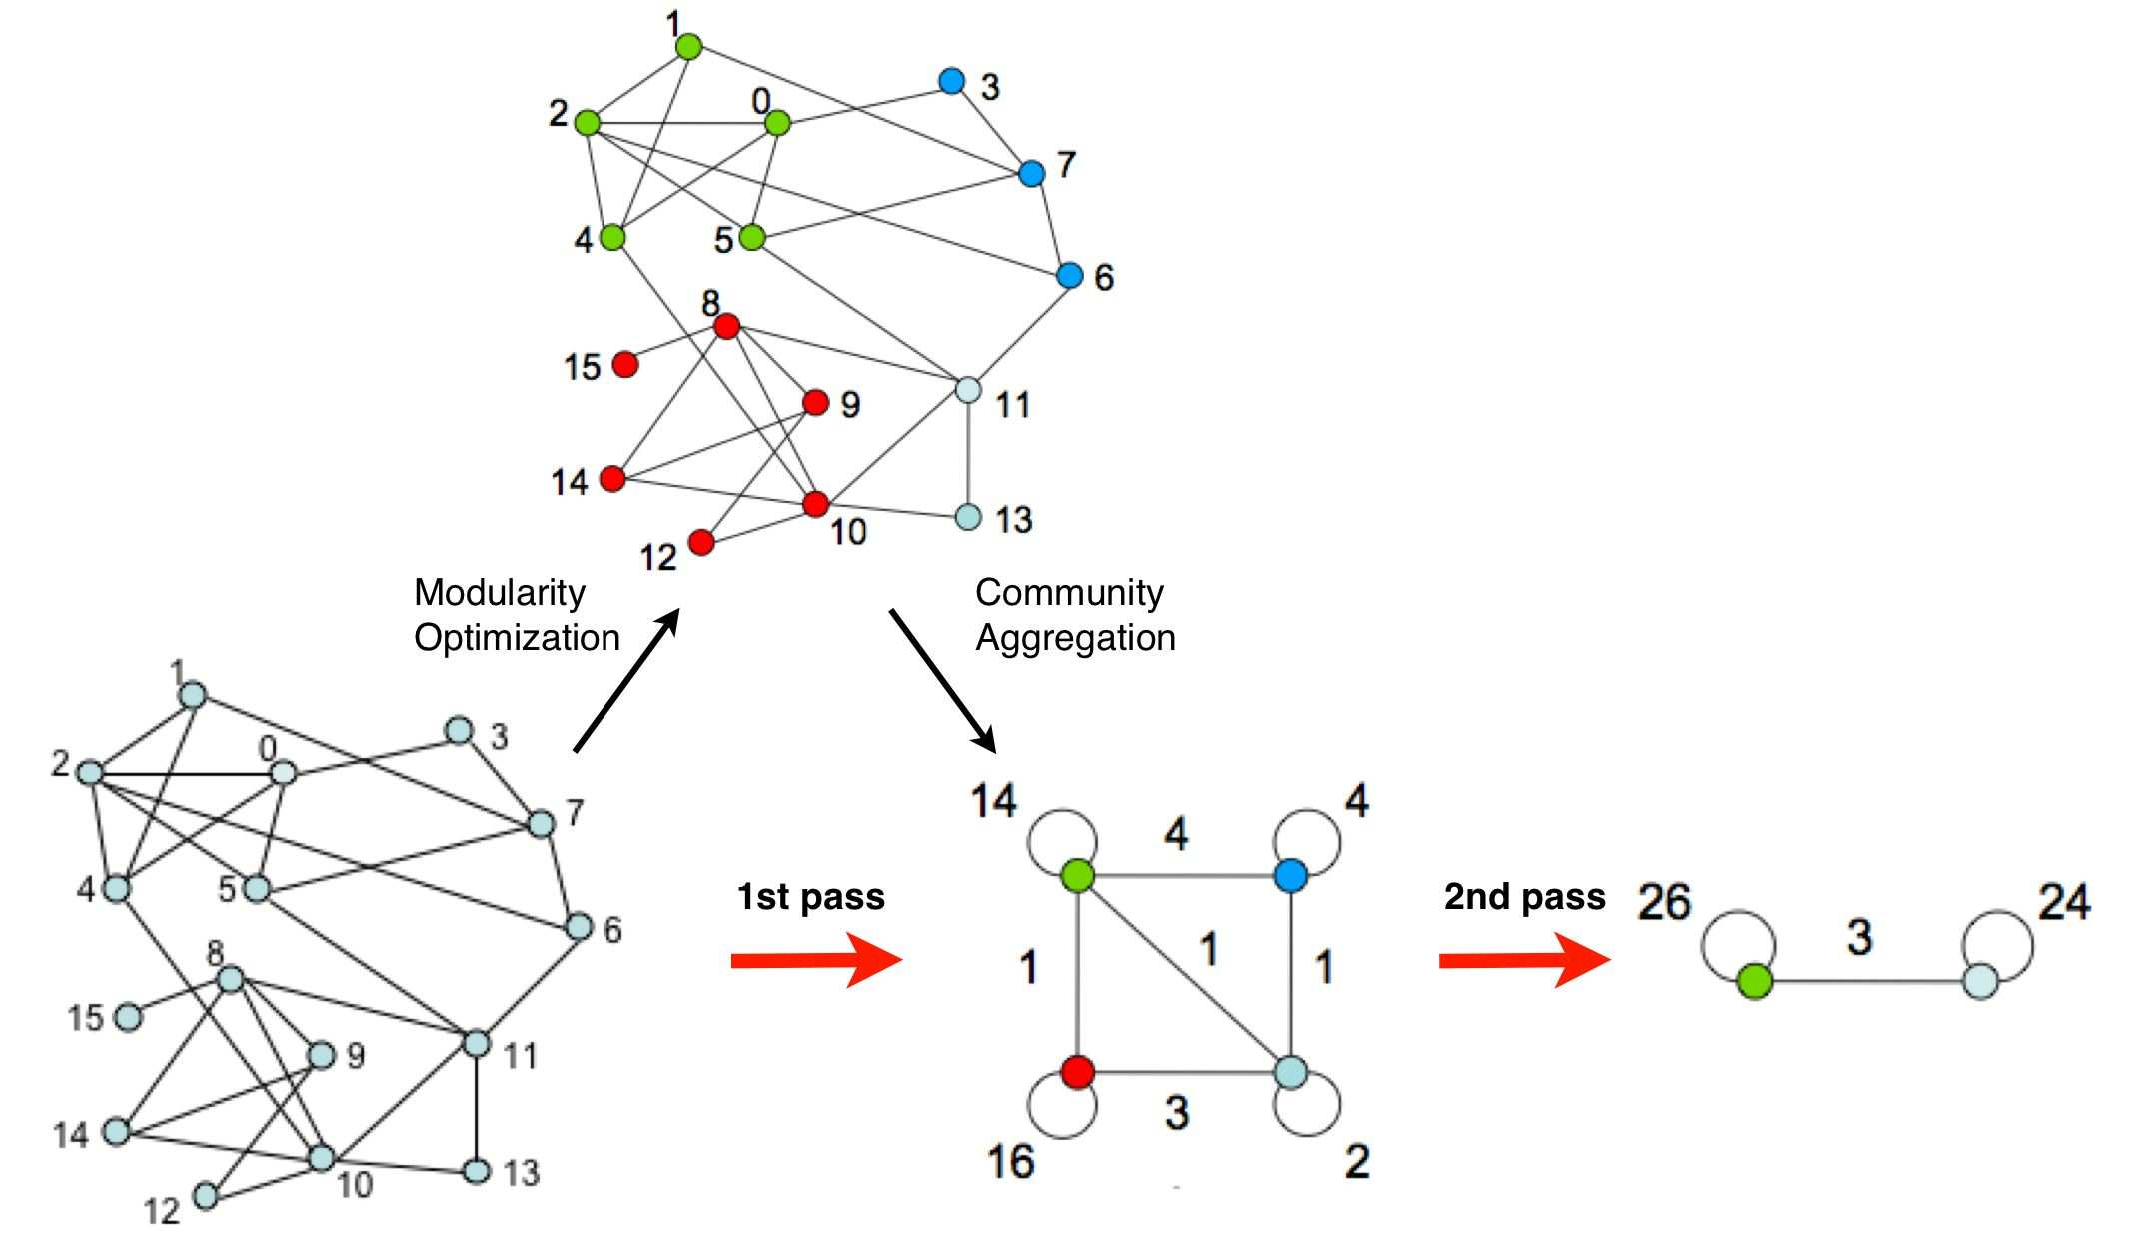
\includegraphics[width=1\linewidth]{0-resources/blondel_scheme}
	\caption{Scheme of the Louvain algorithm. 
	 Given a graph, we first execute the modularity optimization phase that assign each nodes assigned to a community. We have 4 different communities, identified by the colours. Then we perform the communities aggregation phase to create a new graph based on the communities found. After that, the first pass is finished and we repeat these steps until we have an improvement in modularity.This image is reprinted from \cite{Blondel_2008}.}
	\label{fig:blondelscheme}
\end{figure}
We can use the equations (\ref{ModularityC}) to calculate the modularity in current configuration $Q_{i\rightarrow c_i}$ and the modularity $Q_{i\rightarrow c_j}$ in the configuration where $i$ is assigned to $c_j$ and compare the difference, but this is quite inefficient. Instead, we can calculate directly  $\Delta Q_{i \rightarrow c_j}$ as:
\begin{equation}\label{delta_q}
\Delta Q_{i \rightarrow c_j} = \frac{l_{i\rightarrow c_j} - l_{i\rightarrow c_i / \{i\}}}{2|V|} + k_i \frac{k_{c_i / \{i\}} - k_{c_j}}{4|V|^2}
\end{equation}
where $l_{i\rightarrow c_j}$ is the sum of edges that connect $i$ to the community $c_j$, $k_i$ is the weight of the nodes $i$ and $k_{c_j}$ is the weight of the community $c_j$.
Then we define the subset $Z_i$ the set of community $c_z$ with $z \in N(i)$ such that:
\begin{align}
\Delta Q_{i \rightarrow c_z} \geq \Delta Q_{i \rightarrow c_j} && \forall j \in N(i)
\end{align}
If there is more than one community in the group, one community $c_z^*$ is selected using a braking rule, otherwise we pick the only community in $Z_i$. If $\Delta Q_{i \rightarrow c_z^*} > 0$, we move the node $i$ to the community $c_z^*$. \\
This process is applied sequentially on all nodes, and it is repeated while modularity score increases. When no more improvement can be achieved, the second phase starts. In this phase a new network was created from the results of the previous phase: in the new graph, the nodes are the communities found, and the edge between them are given by the sum of the links between nodes that belong to the corresponding communities (edge between nodes in the same communities lead to self-loop). Then we reapply the first step and then the second one until no more improvement is obtained. An example of the algorithm is shown in the Figure \ref{fig:blondelscheme}.
The complexity of this algorithm is $O(m)$ where $m$ is the number of the edges of the graph, due to the fact that we can compute the
gains in modularity for each neighbour easily. Respect to the previous approach, this techniques reaches the goal of the execution in linear time. Indeed, this algorithm can create an entire hierarchy of partitions and this can be useful to avoid the resolution limit problem: we can analyze in the dendrogram the intermediate solutions to observe its structure with the desired resolution \cite{Blondel_2008}.
\subsection{Pruning}\label{prun}
This algorithm is quite efficient even in the first formulation, but large networks requires improvements to be executed quickly. The parallel techniques are very useful for this task and it will be presented in the next chapter. Now we focus on a method that speeds up the computation in the sequential field but that is also suitable in parallel.\\
The first optimization phase is the most time consuming one \cite{Blondel_2008}, requiring about 80\% of the time \cite{wickramaarachchi2014fast}. To reduce the impact of this first phase, in literature were proposed various approach. For example, in \cite{rand}, V. A. Traag proposed to randomize the choice of the community to which assign the nodes. The idea behind these technique is that the nodes that are close to each other tend to be in the same community, so the randomization tend to assign a node to a "good" community. This technique performs well sequentially if the graph has a community structure well defined. Instead, in parallel behaviour, this method doesn't perform well due to the fact that nodes change communities simultaneously: this may lead to a convergence problem and there is no way to prevent simultaneous swaps without introducing some overhead. For this reason, we choose another technique more parallel friendly, introduced by Ozaki et. al \cite{pruning}. Now we present this simple and efficient technique of optimization for this algorithm that doesn't afflict the quality of the partitions. This method makes a pruning of the nodes in the optimization phase in order to compute the maximum delta modularity for only the nodes that have the potential to change community.
Every time a node $i$ changes community from $X$ to $Y$, it affects the $\Delta Q$ of its neighbourhood and all nodes linked and in $X$ and $Y$. Referring to (\ref{delta_q}), we describe all these cases:
\begin{itemize}
	\item Nodes in $X$ that aren't connected to $i$:  for those nodes, the value of $\Delta Q_X$ increase because of the degree of the community $k_X$ decrease without affecting the value of $l_X$.
	\item Nodes in $Y$ that aren't connected to $i$: for those nodes, the value of $\Delta Q_Y$ decrease because the degree of the community $k_Y$ increase without affecting the value of $l_Y$.
	\item  Nodes that are linked to a node in $X$, but not to $i$: for those nodes, the value of $\Delta Q_X$ increase because of the degree of the community $k_X$ decrease without affecting the value of $l_X$.
	\item  Nodes that are linked to a node in $Y$, but not to $i$: for those nodes, the value of $\Delta Q_Y$ decrease because the degree of the community $k_Y$ increase without affecting the value of $l_Y$.
	\item Nodes that are linked to $i$ in $X$:
	in this case both $k_X$ and $l_X$ decrease for $\Delta Q_X$..
	\item Nodes that are linked to $i$ in $Y$:
	in this case both $k_Y$ and $l_Y$ increase for $\Delta Q_Y$.
	\item Nodes that are linked to $i$ but that are not either in $X$ or in $Y$:
	in that case afflict both $\Delta Q_X$ and $\Delta Q_Y$ (increase $k_X$, $l_X$, $k_Y$ and $l_Y$).
\end{itemize} 
The nodes considered in first and the fourth case, doesn't have the potential to change community: in the first case one increase the value of $\Delta Q_X$ that is the maximum (because they are already in the community $X$); in the fourth case one decrease the values of $\Delta Q_Y$ that aren't the maximum (because they are not in the community $Y$). In all other cases, there is a chance that some nodes change community. In the Figure \ref{fig:pruning}, the white nodes are the nodes that doesn't have the potential to change community, instead the black and striped ones are the ones that may have. Considering only these nodes, the computation time will be reduced without reducing the quality of the partition.
\begin{figure}
	\centering
	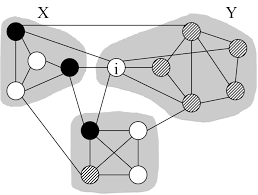
\includegraphics[width=0.7\linewidth]{0-resources/pruning}
	\caption{Example of graph where the nodes $i$ changed community from $X$ to $Y$. The black and striped nodes are the ones with the potential of change community; the white one doesn't have this potential. The pruning technique consider only the black nodes, because considering also the striped ones introducing overhead. This image is reprinted from \cite{pruning}.}
	\label{fig:pruning}
\end{figure}\\
The optimization proposed by Ozaki et. al consists in creating a set of nodes during the iteration of the optimization that will be analyzed in the next step: at the start of the optimization phase, an empty set $S$ is created and every time a node $i$ changes its community, all nodes in its neighbourhood that doesn't belong to the new community are added to $S$. The next iteration considers only the nodes in $S$ and the process is iterated. They consider only one of the four previous categories of nodes: this is because calculating all nodes (explicitly the ones in the second and third group) introduce overhead and this group is the most influential for $\Delta Q$ \cite{pruning}. The selected nodes to be add to $S$ are the black one in the Figure \ref{fig:pruning}. 
The experimental result show that reduce the computational time by up to 90\% compared with the standard Louvain algorithm. In terms of accuracy, surprisingly, the modularity is almost the same,  not only the final one, but also the transition of the modularity during the iterations \cite{pruning}. 
\subsection{Parallel Implementations}\label{parallel-imp}
Now we present various approaches that were used in literature to improve the performance of the Louvain algorithm. We can divide the parallelization techniques
in two different classes: the coarse-grained approach and the fine-grained approach.
The methods in the first-class divide the nodes in some sets and they
are processed independently in parallel for each set. The optimization phase of nodes in the same set are executed sequentially. When all sets are analyzed,
the algorithm merges the results for the next phase. Instead, the second approach
considers each node independently. The community that gives the best modularity for each node is calculated simultaneously and, when all of this values are calculated, we update the communities still in parallel: therefore the decision of the new community for each node is
based on the previous global configuration. Wickramaarachchi et al. \cite{wickramaarachchi2014fast} proposed one of
the first coarse-grained algorithms: in the first iteration, the algorithm partition the graph
in subgraphs and the execution is performed simultaneously and independently
on each partition. Edges that cross the partition are ignored. In terms of quality,
they showed that ignoring cross partition edges does not impact the quality
of the final result.\\
In 2015, both Staudt and Meyerhenke  \cite{staudt2015engineering} and Lu et al. \cite{lu2015parallel} proposed an fine-grained implementation based on OpenMP. To compute $Q_{i \rightarrow c_j}$ for each node $i$ and each community $c_j$ in neighbourhood of $i$ , the algorithm  must calculate $l_{i\rightarrow c_j}$(i.e. the sum of edges that connect $i$ to the community $c_j$ ). These values may change in every new configuration: for this reason, we must have a method to get them fast. In \cite{staudt2015engineering}, they try to associate each node with a map in which the edge weight to neighbouring communities was stored and updated when node moves occurred, but they discover that introduced too much overhead.
Instead, recalculating the weight to neighbour communities each time a node is evaluated turned out to be faster. Therefore, they proposed to use a \verb|map| for each node as an accumulator of his edges to calculate every $l_{i\rightarrow c_j}$. In contrast, the total weights of each community $k_{c_j}$ is stored and updated every time nodes change community. 
This algorithm obtains a speed-up to a factor of 9 with the same quality of the sequential algorithm. The same scheme is used in \cite{lu2015parallel} and they obtain a speed-up to a factor of 16.
This algorithm also highlights a problem of the fine-grained approach: as we can see in the Figure \ref{fig:swap} at the case 1a, neighbouring singleton vertices can simultaneously moving to each others communities if they have the same modularity score. To avoid this problem, they define a rules that say: if a vertex $i$ which is in a community by itself $c_i$ decides to move to another community $c_j$  which also contains only one vertex $j$, then that move will be performed only if $c_j < c_i$. A similar heuristic was used as breaking rules to determine the new community for the nodes: as we see in the in the Figure \ref{fig:swap} at the case 2b, it will improve convergence and permit to avoid local maxima.
\begin{figure}
	\centering
	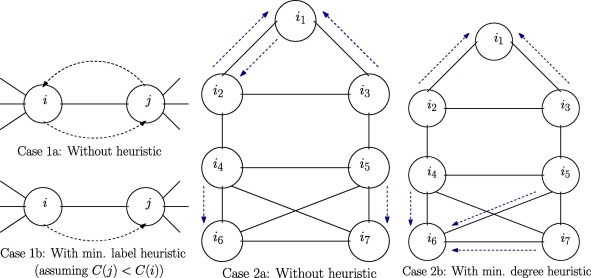
\includegraphics[width=1\linewidth]{0-resources/swap.jpg}
	\caption{ Examples of cases which can be handled by using the minimum labelling heuristic. This image is reprinted from \cite{lu2015parallel}.}
	\label{fig:swap}
\end{figure}\\
A more complex schema was proposed by Que et al. \cite{que2015scalable}: they proposed an algorithm based on a communication pattern that permits to propagate the community state of each node. 
Due to his complex behaviour, this schema is hard to implement on the GPU. \\
Forster in \cite{forster2016louvain} presented a GPU implementation based on the first two previous OpenMP version: he reports a speed-up to a factor of 12 respect to the OpenMP version, but, in the paper, there isn't information about the quality of the partition. Following, the algorithm proposed form Naim et al. \cite{naim2017community} parallelize the hashing of the edges both in optimization and also in the aggregation phase. In addition, they partitioning the vertices into subsets on their degrees to obtain an even load balance between threads.
A different implementation was proposed by Cheong et al. \cite{cheong2013hierarchical}: it is a multi-GPUs implementation that used a coarse grain model between the GPUs and then a fine grain model for the computation of the modularity of each sub-graphs. This algorithm its also peculiar because doesn't use hashing to calculate the modularity: it creates a neighbour community list for each node, sort every list and then sum up the value. In the test with 4 GPUs, this multiple GPUs version is about 3.5 times faster respect to the single GPU version but also reports a loss of up to 9\% in modularity.